\chapter{Heisenberg-Limited Atom Clocks Based on Entangled Qubits}
\label{ch:Kessler2014}
% From \cite{Kessler2014}
%%%%%%%%%%%%%%%%%%%%%%%%%%%%%%%%%%%%%%%%%%%%%%%%

%%%%%%%%%%%%%%%%%%%%%%%%%%%%%%%%%%%%%%%%%%%%%%%%%%%%%%%%%%%%%%%%%%%%%%%%%%%%%%%%%%5
%%%%%%%%%%%%%%%%%%%%%%%%%%%%%%%%%%%%%%%%%%%%%%%%%%%%%%%%%%%%%%%%%%%%%%%%%%%%%%%%%%5
\section{Introduction}
%%%%%%%%%%%%%%%%%%%%%%%%%%%%%%%%%%%%%%%%%%%%%%%%%%%%%%%%%%%%%%%%%%%%%%%%%%%%%%%%%%5
%%%%%%%%%%%%%%%%%%%%%%%%%%%%%%%%%%%%%%%%%%%%%%%%%%%%%%%%%%%%%%%%%%%%%%%%%%%%%%%%%%5
Currently, atomic clocks based on optical transitions achieve the most
precise \cite{Nicholson2012, Bloom2013, Lemke2009} and accurate \cite{Chou2010,
Bloom2013} frequency references.
Additionally, the development of optical frequency combs
\cite{Eckstein1978, Reichert2000, Jones2000, Ye2003} -- establishing a coherent
link between the optical and radio frequencies -- enabled the application
of optical frequency standards to a wide range of scientific and technological
fields including astronomy, molecular spectroscopy and global
positioning systems (GPS).

% The improvement of frequency standards using quantum resources, such as
% entanglement, has attracted wide attention in recent years \cite{Buzek1999,
% Andre2004, Rosenband2012, Rosenband2012_numerical}.

The improvement of frequency standards using quantum resources, such as
entanglement \cite{Buzek1999, Andre2004,LouchetChauvet:2010fs,Rosenband2012_numerical,
Borregaard2013_nearHeisenberg},
%, as well as
%schemes consiting of multi-layered interrogation and feedback
%\cite{Rosenband2013, Borregaard2013} 
has been actively explored in recent years. While clock protocols
based on uncorrelated atoms at best achieve a stability scaling
$\propto1/\sqrt{N}$, where $N$ is the number of atoms -- a
scaling commonly known as the standard quantum limit (SQL) \cite{Caves1980} --
the use of entangled resources, in principle, allows one to surpass this limit.
However, a characterization of the improvement obtainable by using entanglement
 requires a detailed investigation of the decoherence present in the system.
 Previous studies have focused on two kind of noise sources: i) single particle
 decoherence resulting from the interaction of the atoms with the environment
 and ii) frequency fluctuations in the laser used to excite the clock transition
 [in the following also referred to as local oscillator (LO)].
  It is well known that fully entangled states (e.g.,
  Greenberger-Horne-Zeilinger (GHZ) states) allow for improved spectroscopic sensitivity, but in the same way
 that these states benefit from their increased sensitivity in the laser
 interrogation, they are generically prone to various types of noise sources
 canceling any quantum gain. It has therefore been long believed that such
 states fail to increase clock stability regardless of the noise model being used
 \cite{Bollinger1996, Wineland1998, Rosenband2012_numerical,Huelga1997}. On the other hand, it has been shown that
for clocks with local oscillator noise limited stability, the use of
moderately squeezed atomic states can yield a modest improvement over the SQL
\cite{Andre2004,LouchetChauvet:2010fs}.
 A recent study demonstrated further that, in principle, highly squeezed states
could achieve Heisenberg-limited stability (i.e., a $1/N$ scaling
with the available resources representing the ultimate limit allowed by the laws
of quantum mechanics \cite{Giovanetti2011}) using a complex adaptive
measurement scheme \cite{Borregaard2013_nearHeisenberg}.
 At the same time, it has been shown that the single particle
 decoherence-limited regime can be reached for long averaging time at
a logarithmic cost in $N$ by interrogating uncorrelated atomic
ensembles for suitably chosen times \cite{Rosenband2013, Borregaard2013}.

In this Letter, we  introduce a protocol involving groups of sequentially larger
GHZ states to estimate local oscillator deviations from the atomic reference in
a manner reminiscent of the phase estimation algorithm \cite{Nielsen_Chuang}.
Furthermore, we unify previous treatments of decoherence for atomic clocks 
and incorporate previous proposals involving uncorrelated atoms to
effectively narrow the LO linewidth \cite{Rosenband2013, Borregaard2013} and thereby identify
 ultimate limits to the stability of atomic clocks based on entangled atoms. We find that for LO-noise limited clocks, the
proposed quantum protocol is found to be nearly optimal, realizing the
Heisenberg limit of clock stability up to a logarithmic correction in the
particle number.
Importantly, it reaches the fundamental noise floor  resulting from
individual dephasing of the clock qubits $N$ times faster than the best known
classical schemes, where $N$ is the total number of particles employed.

%In this Letter, we demonstrate that if the dominating noise is LO noise -- as it is the case in modern atomic clocks -- this limitation can be overcome.  
%As the LO fluctuations affect all clock atoms alike, this perfectly correlated noise does not represent a fundamental limitation in the interrogation process, and can be corrected for in a non-adaptive protocol based on multiple GHZ states of varying size, reminiscent of the phase estimation algorithm  \cite{Nielsen_Chuang}. 
%% The procedure is based on the
%% division of the available clock atoms into successively smaller GHZ groups
%% evolving at different phase velocities during the laser interrogation time. Each
%% GHZ group hereby keeps track of the accumulated phase slips of the next
%% ensemble, thus largely eliminating the problem of uncontrolled slips of the
%% laser phase. This allows us to operate a large part of the available resources
%% in a fully entangled state, reaching near-Heisenberg-limited spectroscopy for
%% LO-noise-limited optical clocks,  with an $\mathcal O(\sqrt N/ \mathrmrm{log}(N))$
%% stability improvement over the SQL. 
%We provide the full quantum mechanical
%derivation of this result, 
%% in a feedback analysis, 
%taking into account all relevant noise sources and optimizing over all free
%parameters of the scheme.
%We investigate the limiting factors of atomic clock stability over different
%time scales, and provide a detailed comparison with classical clock protocols.
%The proposed quantum protocol is found to be optimal, realizing the Heisenberg limit of laser stability up to a logarithmic correction in the particle number. It reaches the fundamental noise floor resulting from individual dephasing of the clock qubits $\sim N$ times (with $N$ being the total number of particles employed) faster than the best classical schemes.

The central idea of our approach can be understood as follows.
In modern atomic clocks, the frequency of a LO is locked to an ultra-narrow
 transition of the clock atoms serving as the
frequency reference.
The long-term stability  of such a clock after a given total averaging time
$\tau$ is directly related to the precision by which the accumulated laser phase
relative to the atoms can be determined. To this end, the phase is repeatedly
measured in a standard Ramsey protocol \cite{Ramsey1950}:
Using the LO, the clock qubits are prepared in a superposition of $\ket 1$ and
$\ket 0$, denoting the levels of the clock transition. After the qubits evolve
freely for a time $T$ (Ramsey interrogation time), they are subsequently
measured in an orthogonal basis ($\ket \pm \equiv \ket 1 \pm\ket 0$), which
yields an estimate of the accumulated phase difference between the LO and the
atomic frequency reference.
It is known, that since each of these Ramsey sequences introduces measurement
noise, it is optimal to extend the Ramsey time $T$ 
to its maximum value $T\rightarrow\tau$ \cite{Braunstein:1992bx}.

A single GHZ state consisting of $N$ entangled atoms -- whose state after the
interrogation is $\ket{\mathrm{GHZ}}_T \propto \ket{0}^{\otimes N} + \mathrm{exp}(-i
N\Phi_{\mathrm{LO}}) \ket{1}^{\otimes N}$ -- accumulates the laser phase (denoted
by $\Phi_{LO}$) $N$ times faster than an uncorrelated state, allowin a more precise
phase measurement \cite{Giovanetti2011}. However, fluctuations in the
laser frequency renders the laser phase a
random variable with a probability distribution that grows in width as we
increase  the Ramsey time $T$.
Whenever the laser phase realized in a particular Ramsey cycle induces a full
phase wrap on the state [i.e., the atomic phase $N \Phi_{LO}\notin[-\pi,\pi)$]
a subsequent measurement yields a $2\pi$ error in the estimation. For a single GHZ
state, this accounts for a strict limitation on the maximally allowed Ramsey
time in order  to limit the initial variance of $\Phi_\mathrm{LO}$, and the resulting
laser stability is found to yield no improvement over classical protocols 
\cite{Wineland1998}.

% cause large variations of the phase picked up by the interrogating state in
% the different cycles. Whenever these fluctuations induce a full phase wrap on
% the state [i.e., the atomic phase $N \Phi_{LO}\notin[-\pi,\pi)$] a subsequent
% measurement yields no useful information on the true laser phase due to the
% periodicity of the exponential. For a single GHZ state this accounts for a
% strict limitation on the maximally allowed Ramsey time in order  to limit the
% initial variance of the distribution of $\Phi_\mathrm{LO}$, and thus a resulting
% laser stability that is found to yield no improvement over classical protocols
%  \cite{Wineland1998}.


To address this problem, we use a protocol involving an incoherent version of
the \textit{phase estimation algorithm} \cite{Nielsen_Chuang}, similar to the
one outlined in \cite{Giovannetti2006} but adapted to be applicable also when
the frequency fluctuates and phases exceed $2\pi$. The
phase estimation algorithm has recently been successfully applied experimentally
for global interferometric phase estimation \cite{Higgins2007,Mitchell2005}, and
its use in clock synchronization protocols has been discussed \cite{Burgh2005}.
Here, we demonstrate how the same techniques can be applied to
guarantee optimal laser stability by allowing the Ramsey interrogation
time to be extended to its maximum value.

\begin{figure}
\centering
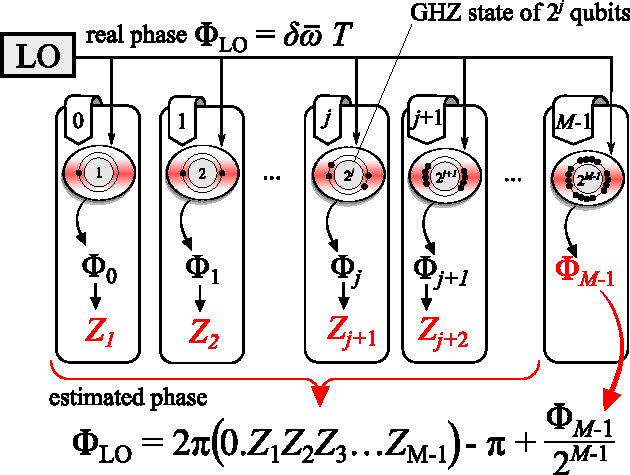
\includegraphics[width=0.8\textwidth]{./figs_Kessler2014/fig2.pdf}
\caption
[GHZ cascade]
{
\label{fig:phase_estimation}
The proposed clock operation scheme employs $M$ different groups of clock atoms
prepared in correlated states of varying size to interrogate the relative phase
$\Phi_\mathrm{LO}$ of the LO field.
A single group $j$ contains $n_0$ independent instances of GHZ-like states, each
entangling $2^j$ qubits, and therefore accumulating a phase $\Phi_j = 2^j
\Phi_\mathrm{LO} \mod [-\pi,\pi]$ during a single cycle. Each group is then used
to measure this phase, which gives a direct estimate on the digit $Z_{j+1}$ in a
binary representation of the LO phase
$(\Phi_\mathrm{LO}+\pi)/2\pi=(0.Z_1Z_2Z_3\hdots)$,
subsequently used to feedback the LO frequency.
}
\end{figure}

Let us assume, for the moment, that the accumulated laser phase after the
interrogation time $T$ lies in the interval $\Phi_\mathrm{LO}\in[-\pi,\pi)$, and
has an exact binary representation $(\Phi_\mathrm{LO}+\pi)/2\pi= \sum_{j=1}^M Z_j/
2^{j}$, with digits $Z_j\in \{0,1\}$ (both conditions will be relaxed below).
One can then readily show that a GHZ state consisting of $2^{M-1}$ atoms picks
up the phase $\Phi_{M-1} = 2^{M-1} \Phi_\mathrm{LO}  ~\mathrm{mod}~ [-\pi,\pi) = \pi
(Z_M-1)$. Thus, by measuring if the phase is $0$ or $\pi$, the last digit of the
laser phase can be determined. However, without
the remaining digits this information is
useless.
In our protocol, these digits are found by an additional, simultaneous
interrogation with successively smaller GHZ states of $2^{M-2},2^{M-3},\hdots$
entangled atoms (see \reffig{fig:phase_estimation}). Each of these states
picks up a phase proportional to its size  $\Phi_{j} = 2^{j}
\Phi_\mathrm{LO}~\mathrm{mod}~ [-\pi,\pi)$, and this
phase gets a contribution of $\pi (Z_j-1)$.
By distinguishing whether the phase is shifted by $\pi$ or not, we can 
determine the value of the bit $Z_j$.
The combined information provides an estimate with an accuracy given by the
largest GHZ state, while the cascade increases the total number of atoms
employed only by a factor of two: $\sum_{j=0}^{M-1} 2^j \approx
2^{M}=2\times2^{M-1}$.

However, in the limit of large averaging times, the assumption
$\Phi_\mathrm{LO}\in [-\pi,\pi)$ is not justified anymore. Here, the optimal
Ramsey time $T\sim\tau$ can attain values that induce phase wraps of the laser
itself, causing the binary representation of the laser phase to contain digits
$Z_j\neq0$ for $j\leq0$, which are inaccessible to the technique discussed
above.
To overcome this, we extend the cascade to
the classical domain, and employ additional groups of {\it uncorrelated}
atoms that interrogate the laser with successively decreasing interrogation times, or
alternatively, using dynamical decoupling techniques \cite{Rosenband2013,
Borregaard2013,ddc}. Each of these ensembles acquires a phase that is
reduced by multiples of two from the laser phase, and thus, following the
arguments from above, allows one to gain information on the digits
$Z_j$ with $j\leq0$.
The information of all digits combined provides the total number of phase wraps,
which in turn yields a Heisenberg-limited estimate of the laser phase.
By this, the protocol effectively eliminates all limitations
arising from the LO noise, and allows the Ramsey time to extend to its optimal
value.

 
% This paper is organized as follows. In Section~\ref{sec:EC} we provide an
% executive summary of the proposed clock operation scheme and the main results of
% our feedback analysis. This Section is self-contained, and can be read without
% consulting the following part of the paper.
% For the interested reader, the subsequent Sections provide the full details of
% our analysis. In Section $\hdots$

% It is a long standing view that GHZ-states cannot increase clock stability due
% to their increased susceptibility to phase slips in the presence of $1/f$-type
% local oscillator noise. \cite{Wineland1998}



%%%%%%%%%%%%%%%%%%%%%%%%%%%%%%%%%%%%%%%%%%%%%%%%%%%%%%%%%%%%%%%%%%%%%%%%%%%%%%%%%%5
%%%%%%%%%%%%%%%%%%%%%%%%%%%%%%%%%%%%%%%%%%%%%%%%%%%%%%%%%%%%%%%%%%%%%%%%%%%%%%%%%%5
\section{Feedback loop}
%%%%%%%%%%%%%%%%%%%%%%%%%%%%%%%%%%%%%%%%%%%%%%%%%%%%%%%%%%%%%%%%%%%%%%%%%%%%%%%%%%5
%%%%%%%%%%%%%%%%%%%%%%%%%%%%%%%%%%%%%%%%%%%%%%%%%%%%%%%%%%%%%%%%%%%%%%%%%%%%%%%%%%5
In the following, we provide a derivation of the above results
combined with feedback analysis that allows us to characterize
the achievable stability of a clock using our protocol. Modern
clocks periodically measure the fluctuating LO frequency $\omega(t)$ against the
frequency standard $\omega_0$ of the clock atoms to
obtain an error signal.
After each Ramsey cycle of duration $T$ [i.e., at times $t_k=kT$
($k=1,2\hdots$)], the measurement data yield
 an estimate of the relative phase, $\Phi_\mathrm{LO}(t_k) =
\int_{t_k-T}^{t_k}\d{t}[\omega(t) - \omega_0]$, accumulated by the LO.
This estimate in turn is used to readjust the frequency of the LO:  $\omega(t_k)
\rightarrow \omega(t_k) - \alpha\Phi^\mathrm{est}_\mathrm{LO}(t_k)/T$, where
$\Phi^\mathrm{est}_\mathrm{LO}(t_k)$ represents a suited estimator of the phase
$\Phi_\mathrm{LO}(t_k)$ \footnote{Alternatively, it is also possible to perform direct phase
feedback.}, and $\alpha < 1$ is an suitably chosen
gain.
%Phase feedback
%is chosen since it performs better in the presence of white noise
%\cite{Bollinger1996}, but one can use frequency
%feedback and achieve the same stability up to a constant factor.

The stability of the actively stabilized LO, after a total averaging time
$\tau$, is characterized by the Allan deviation (ADEV) which is directly
proportional to the measurement uncertainty $\Delta\Phi_\mathrm{LO}(t_k)$ after
each Ramsey cycle (see Appendix \ref{app:Kessler2014}),
\bel
	\label{eq:Allan-variance}
	\sigma_y(\tau) \equiv \frac{1}{\omega_0 \tau}
	\sqrt{\sum_{k = 1}^{\tau/T}\sum_{l = 1}^{\tau/T}
	T^2\ev{\delta\bar\omega_k\delta\bar\omega_l} }
	\approx
	 \frac{1}{\omega_0\sqrt{\tau T}} \Delta\Phi_\mathrm{LO}(T).
%  	 =
% 	\frac{1}{\omega_0^2\tau T} \frac{(\Delta\Phi_{M-1})^2}{D^{2M-2}}
% 	=:
% 	\frac{\gamma}{\omega_0^2 \tau} S^2(\gamma T,D,M,N)  ,
\eel
Here, $\delta\bar\omega_k = \Phi_\mathrm{LO}(t_k)/T$ is the average detuning of the
(stabilized) LO during the $k$th cycle. {%
 To obtain \refeq{eq:Allan-variance}, we use the fact that after the frequency
 feedback the detuning averages become approximately uncorrelated for realistic
 laser spectra, $\ev{\delta\bar\omega_k \delta\bar\omega_l} \approx
 \ev{\delta\bar\omega^2}\delta_{kl}$ \cite{Borregaard2013,
 Andre2005,Bloom2013}}.
%It has been shown that, if the frequency noise spectrum of the free running LO,
%$S_\omega(f)$, is less divergent than $\mathcal{O}(1/f^2)$ as  $f\rightarrow 0$,
%then the low-frequency part of the frequency noise spectrum of the actively
%stabilized LO $S^\mathrm{st}_\omega(f)$ is dominated by white noise originating
%entirely from measurement uncertainties \cite{Borregaard2013, Andre2005}.
%Since realistic laser noise spectra -- being dominated by white and $1/f$-noise
%(electronic flicker noise) \cite{Bishof2013} -- fulfill this condition,
%different Ramsey cycles are independent, and write the covariance as
%$\ev{\delta\bar\omega_k \delta\bar\omega_l} = \ev{\delta\bar\omega^2}\delta_{kl}
%= (\Delta \Phi_\mathrm{LO})^2\delta_{kl}/T^2$, which results in the right hand
 %side of \refeq{eq:Allan-variance}.
Other noise sources (such as the bias of the linear estimator, the Dick effect,
or a sub-optimal gain $\alpha$ \cite{Santarelli1998}) are not fundamental, and
neglected in the following.


%%%%%%%%%%%%%%%%%%%%%%%%%%%%%%%%%%%%%%%%%%%%%%%%%%%%%%%%%%%%%%%%%%%%%%%%%%%%%%%%%%5
%%%%%%%%%%%%%%%%%%%%%%%%%%%%%%%%%%%%%%%%%%%%%%%%%%%%%%%%%%%%%%%%%%%%%%%%%%%%%%%%%%5
\section{Spectroscopic nosies}
%%%%%%%%%%%%%%%%%%%%%%%%%%%%%%%%%%%%%%%%%%%%%%%%%%%%%%%%%%%%%%%%%%%%%%%%%%%%%%%%%%5
%%%%%%%%%%%%%%%%%%%%%%%%%%%%%%%%%%%%%%%%%%%%%%%%%%%%%%%%%%%%%%%%%%%%%%%%%%%%%%%%%%5

For small values of the accumulated Ramsey phase, the ultimate precision by
which this phase can be estimated is determined by the Cram\'{e}r-Rao bound
\cite{Rao1945,Giovanetti2011} which 
links the estimation error to the quantum Fisher information (QFI)
$\Delta\Phi_\mathrm{LO} \sim 1/\sqrt{\mathcal F}$ (for a review, see
\cite{Giovanetti2011}). The QFI, $\mathcal F$, is maximized, e.g., by the use of
GHZ states for which $\mathcal F \sim N^2$.
In clock stabilization, however, the LO frequency fluctuations account for the
fact that the accumulated Ramsey phase is a random variable which can obtain
large values, inherently violating the small phase assumption of the
Cram\'{e}r-Rao bound.
% A phase wrap error occurs whenever $\Phi(t_k)$ falls outside the interval
% $[-\pi,\pi)$ at the end of the $k$th cycle which can not be detected in a
% standard Ramsey measurement.
In particular for a single GHZ states, phase wraps of the atomic phase,
$\Phi(t_k)=N \Phi_\mathrm{LO}(t_k)\notin[-\pi,\pi)$, cannot be detected.
Consequently, the cycle time $T$ has to be
chosen such that the prior distribution of $\Phi(t_k)$ is well localized
within $[-\pi,\pi)$.
This limits the maximally allowed Ramsey time to a value $T_\mathrm{max}
\sim\gamma_\mathrm{LO}^{-1}/N^2$ (see 
Appendix \ref{app:Kessler2014}), where we assumed a white frequency noise
spectrum of the LO, $S_\omega(f) = \gamma_\mathrm{LO}$ (for $1/f$-noise one finds the less stringent
condition $T_\mathrm{max} \sim\gamma_\mathrm{LO}^{-1}/N$). In most cases, this value
lies below the optimal (i.e., maximal) value implied by
\refeq{eq:Allan-variance} $T\sim\tau$, resulting in a laser stability for GHZ
states which shows no improvement over the stability achieved with uncorrelated
atoms \cite{Wineland1998, Rosenband2012_numerical}.

However, unlike the individual particle noise resulting in the finite atom
linewidth $\gamma_\mathrm{ind}$, the LO frequency fluctuations affect all clock
atoms alike, and this \textit{collective noise} does not represent a fundamental
metrological limitation.
Ee can use a cascade of GHZ states of varying size to measure the
$\Phi_\mathrm{LO}$ in a binary representation, as discussed above.
In general, the phase does not have an exact binary representation ending at the
digit $Z_{M}$. We therefore employ $n_0$ duplicates  at each level of the
cascade (as opposed to sequential procedure suggested in \cite{Giovannetti2006})
($n_0 =N/\sum_{j=0}^{M-1} 2^j \approx N/2^M$) to improve the precision.
 In the case where all digits $Z_j$ ($j=1\dots, M-1$) are determined correctly
 according to the relation
\bel
Z_j =
[2(\Phi_{j-1}+\pi) - (\Phi_j + \pi)]/2\pi,
\eel
the last group ($j=M-1$) then yields a Heisenberg-limited estimate of
the LO phase with accuracy $(\Delta\Phi_\mathrm{LO})_\mathrm{pr} =
1/(2^{M-1} \sqrt{n_0}) = 2\sqrt{n_0}/N$.

%%%%%%%%%%%%%%%%%%%%%%%%%%%%%%%%%%%%%%%%%%%%%%%%%%%%%%%%%%%%%%%%%%%%%%%%%%%%%%%%%%5
%%%%%%%%%%%%%%%%%%%%%%%%%%%%%%%%%%%%%%%%%%%%%%%%%%%%%%%%%%%%%%%%%%%%%%%%%%%%%%%%%%5
\subsection{Phase estimation with multiple GHZ groups}
%%%%%%%%%%%%%%%%%%%%%%%%%%%%%%%%%%%%%%%%%%%%%%%%%%%%%%%%%%%%%%%%%%%%%%%%%%%%%%%%%%5
%%%%%%%%%%%%%%%%%%%%%%%%%%%%%%%%%%%%%%%%%%%%%%%%%%%%%%%%%%%%%%%%%%%%%%%%%%%%%%%%%%5
%{\it Cascaded GHZ.}---

%Let us assume for the moment that the prior distribution of the LO phase $\Phi_\mathrm{LO}$ after the
%Ramsey time is localized in $[-\pi,\pi)$ (we will relax this condition below), such that we can write $(\Phi_\mathrm{LO}+\pi)/
%2\pi= \sum_{j=1}^\infty Z_j/ 2^{j}\equiv0.Z_1Z_2Z_3\hdots$

%0.Z_1Z_2Z_3\hdots$. 
%Then we can
%represent the  phase we want to estimate as a binary fraction
%$(\Phi_\mathrm{LO}+\pi)/2\pi= \sum_{j=1}^\infty Z_j/ 2^{j}\equiv
%0.Z_1Z_2Z_3\hdots$, with digits $Z_j\in\{0,1\}$.


%We imagine dividing the $N$ qubits available into $M$ groups
%($j=0,1\dots M-1$), each containing $n_0$ independent instances of  $2^j$ number of
%qubits entangled in a GHZ state, $\ket{\mathbf{1}}_j + i \ket{\mathbf{0}}_j
%\equiv\ket{0}^{\otimes{2^j}} + i\ket{1}^{\otimes{2^j}}$ ($n_0 =
%N/\sum_{j=0}^{M-1} 2^j \approx N/2^M$), as shown in \reffig{fig:phase_estimation}.
 %Subsequently, the LO field is
% (with average detuning $\delta\bar\omega$)
%interrogated by all entangled states simultaneously  in a Ramsey cycle of length
%$T$, using the technique described in \cite{Bollinger1996}.
%After this interrogation the respective GHZ states are given as
%$\ket{\mathbf{1}}_j + i e^{i\Phi_j} \ket{\mathbf{0}}_j $ having accumulated the
%phase 
%\begin{align} \label{eq:EK1}
%\Phi_j =& 2^j \Phi_\mathrm{LO}  ~\mathrm{mod}~ [-\pi,\pi) \\ 
%=&2\pi 
%(0.Z_{j+1} Z_{j+2} Z_{j+3}\hdots)-\pi.
%\end{align}
%The largest group
%$j=M-1$ (i.e., the group with the fastest evolving GHZ states) consequently 
%can estimate $\Phi_{M-1} =2\pi  (0.Z_{M} Z_{M+1} \hdots)-\pi $ with accuracy
%$\Delta\Phi_{M-1} = 1/\sqrt{n_0} $ \cite{Itano1993,fn2}.
%The number of phase slips  $Z_1\hdots Z_{M-1}$ -- necessary to derive an estimate of the laser phase $\Phi_{LO}$ --  subsequently can be measured directly digit by digit from the groups of
%successively smaller GHZ states according to the relation 
%\bel
%Z_j =
%[2(\Phi_{j-1}+\pi) - (\Phi_j + \pi)]/2\pi
%.
%\eel If all digits $Z_j$ are determined correctly this yields a Heisenberg-limited estimate of
%the LO phase with accuracy $(\Delta\Phi_\mathrm{LO})_\mathrm{pr} =
%1/(2^{M-1} \sqrt{n_0}) = 2\sqrt{n_0}/N$, and with a Ramsey time that 
%can exceed the laser noise limit $T_\mathrm{max}$.

However, in general the estimation of the binary digits $Z_j$ is not perfect.
A rounding error occurs whenever $|\Phi_{j-1}^\mathrm{est} - \Phi_{j-1}| > \pi/2$
(where $\Phi_j^\mathrm{est}$ represents a suitable estimator derived from the $n_0$
measurement outcomes), leading to the wrong $Z_j$, and a variance contribution
of $(2\pi 2^{-j})^2$ for $\Phi_\mathrm{LO}$.
We can approximate their total
variance contribution with the sum
 $ 	(\Delta\Phi_\mathrm{LO})^2_\mathrm{re} = P_\mathrm{re}\sum_{j=1}^{M-1}
 	(2\pi 2^{-j})^2
%  	\frac{D}{\pi}\exp\left[-\frac{\pi^2}{D^2}n_0\right] 
%  	\approx 4\pi D^{2M-3}
%  	\exp\left[-\frac{\pi^2}{D^2}n_0\right].
 $, where 
$P_\mathrm{re} = 2\intop_{\pi/2}^{\infty}\d{\phi}
\rho(\phi)$, 
% \bel
% 	\label{eq:p_re}
% 	p_\mathrm{rounding error} = 2\intop_{\pi/2}^{\infty}\d{y} \rho(y) <
% 	2\intop_{\pi/2}^{\infty}\d{y} n_0 e^{-n_0y^2} 
% 	=
% 	\frac{2}{\pi}\exp\left[-\frac{\pi^2}{2^2}n_0\right] \left(1 +
% 	\mathcal{O}\left(\frac{2}{\pi}\right)\right), \qquad \forall j,
% \eel
and $\rho(\phi)$ is the Gaussian probability distribution of the error
$\Phi_j^\mathrm{est} - \Phi_j$ with a width proportional to $1/\sqrt n_0$  
(see Appendix \ref{app:Kessler2014}).
Consequently, rounding errors can be exponentially suppressed by choosing a
sufficiently large value for $n_0$. The total
measurement uncertainty of this estimation scheme is thus
$(\Delta\Phi_\mathrm{LO})^2 = (\Delta\Phi_\mathrm{LO})_\mathrm{pr}^2
+(\Delta\Phi_\mathrm{LO})_\mathrm{re}^2$.
In Appendix \ref{app:Kessler2014}, we show that the optimal allocation of
resources is achieved for the choice $n_{0}^{\mathrm{opt}} \sim
\frac{16}{\pi^2}\log\left(N\right)$, for which rounding errors are negligible,
yielding the total measurement accuracy
 \bel
 \label{eq:M}
\Delta\Phi_\mathrm{LO} \approx (\Delta\Phi_\mathrm{LO})_\mathrm{pr} =
\frac{8}{\pi}\sqrt{\mathrm{log}(N)}/N.
\eel This measurement precision obtains the Heisenberg limit (up to a
logarithmic correction resulting from the cost to suppress rounding errors)
despite it being applicable to a general (typically large) phase.

% \bel
% \tilde\Phi_j = (\Phi_j \mod [-\pi,\pi])= (D^j T\delta\bar\omega \mod
% [-\pi,\pi]),\qquad\qquad \Delta\tilde\Phi_j =
% \frac{1}{\sqrt{n_0}} \quad \forall j\qquad\mathrm{(from MLE)}
% \eel
% where $T$ is the free evolution time (See \reffig{fig:phase_estimation}).
% Its
% uncertainty is a good approximation
% % (strictly speaking, an upper bound) 
% of the uncertainty of $\Phi_\mathrm{LO}$, $\Delta\Phi_\mathrm{LO} =
% \Delta\Phi_{M-1}/D^{M-1}$.
% % \bel
% % 	\Delta\Phi_\mathrm{LO} = \frac{\Delta\Phi_{M-1}}{D^{M-1}}.
% % \eel
% Unfortunately, 

%Note, that this estimation protocol can be understood as an incoherent
%version of the phase estimation algorithm. However, as compared to previous versions of the latter \cite{Geza} the measurement uncertainty is
%reduced by a factor $ \propto 2^{M/2}/\sqrt{\mathrm{log}(N)}$ enabling the full
%quantum gain of our protocol.

So far we have assumed that $\Phi_\mathrm{LO}\in[-\pi,\pi)$ in each cycle.
However, for realistic laser noise spectra there is always a finite probability
that the LO phase $\Phi_\mathrm{LO}$ lies outside the interval $[-\pi,\pi)$ after
the interrogation time. Such phase wraps of the laser phase itself add to the
final measurement uncertainty in \refeq{eq:M} by the amount
$
	(\Delta\Phi_\mathrm{LO})^2_\mathrm{slip} =  (2\pi)^2P_\mathrm{slip}
$,
where 
$P_\mathrm{slip} = 2\intop_\pi^\infty \d{\phi} \rho_\mathrm{LO}(\phi)$,
% \bel
% 	\label{eq:p_slip}
% 	p_\mathrm{slip} = 2\intop_\pi^\infty \d{y} \rho_\mathrm{LO}(y) = 2\intop_\pi^\infty
% 	\d{y} \frac{1}{\sqrt{2\pi (\gamma T)^2}}
% 	\exp\left[-\frac{y^2}{2(\gamma T)^2}\right] = \sqrt{\frac{2}{\pi}}
% 	\frac{\gamma T}{\pi}\exp\left[-\frac{\pi^2}{2(\gamma T)^2}\right] \left(1
% 	+ \mathcal{O}\left(\frac{\gamma T}{\pi}\right)\right),
% \eel
and $\rho_\mathrm{LO}$ is the Gaussian prior distribution of $\Phi_\mathrm{LO}$.
Its width grows with $ \gamma_\mathrm{LO} T$, which puts a constraint on the
maximally allowed Ramsey time $T
\leq\frac{\pi^2}{4}\gamma_\mathrm{LO}^{-1}[\log(\gamma_\mathrm{LO}\tau N)]^{-1}$,
and thus the achievable ADEV $\sigma_y~(\propto 1/\sqrt T)$
 as we demonstrate in Appendix \ref{app:Kessler2014}.

This, however, does not represent a fundamental limitation as we can
extend the scheme by adding additional classical measurements with a shorter
Ramsey periods to assess the number of phase slips of
the laser phase itself $\hdots Z_{-3}Z_{-2}Z_{-1}Z_0$. As demonstrated in
Appendix \ref{app:Kessler2014}, this allows  extending the Ramsey time by a
factor $k$ adding only a negligible number of atoms $N^{*}\approx
\frac{8}{\pi^2} \log\left(k N^2\right)\log_2(k)\ll N$.
% This procedure can be understood as a classical pre-narrowing of the laser
% linewidth before the application of the quantum protocol.

% Using classical techniques the effective laser linewidth can be pre-narrowed
% before application of the proposed quantum protocol. This is achieved in a
% parallel interrogation with classical ensembles that measure the laser phase
% using varying Ramsey times, or alternatively, by employing dynamical
% decoupling techniques \cite{Rosenband2013, Borregaard2013,ddc}.
 % It allows the extension of the Ramsey time by a factor $k$ at negligible cost
 % in total resources $N^{*}\approx \frac{2}{\pi^2} D^2 \log\left(k
 % N^2\right)\log_D(k)\ll N$.
 % As we demonstrate in the SI, this can be understood as an extension of the
 % cascaded interrogation scheme to the classical domain to assess the binary
 % digits left of the point, $Z_j$ ($j<0$), eliminating the threat of
 % unaccounted phase slips of the laser phase.
 
% The Ramsey time is then only limited by individual noise processes resulting
% in the finite linewidth of the clock atoms $\gamma_\mathrm{ind}$ which put a
% fundamental limit on the allowed Ramsey time
% $T\leq\gamma_\mathrm{ind}^{-1}/2^{M-1}$, inversely proportional to the size of
% the GHZ states in group $M-1$.




%However, also here rounding errors do not represent a fundamental limitation. The necessity of using multiple copies $n_0$ can in principle be avoided by a quantum processing step of the clock atom state prior to the measurement. After the the interrogation time T the total state of the system is given as
%\begin{align}
%\Ket{\Psi} =\frac{1}{2^{M/2}}& \left( \Ket{\mathbf0}_0 + e^{i2^0\Phi_\mathrm{LO}}\Ket{\mathbf{1}}_0\right)\left( \Ket{\mathbf0}_1 + e^{i2^1\Phi_\mathrm{LO}}\Ket{\mathbf{1}}_1\right)\hdots\\
%&\left( \Ket{\mathbf0}_{M-1} + e^{i2^{M-1}\Phi_\mathrm{LO}}\Ket{\mathbf{1}}_{M-1}\right),
%\end{align}
%where we defined the logical qubits $\Ket{\mathbf0}_j = \Ket{0}^{\otimes 2^j}$ ($\Ket{\mathbf1}_j = \Ket{1}^{\otimes 2^j}$), according to the different GHZ groups. In the pathological case that $\phi_\mathrm{LO}$ has an exact $M$ bit binary representation, one readily shows that application of the inverse quantum Fourier transformation $U_\mathrm{QFT}^{-1}$ on the logical qubit state yields
%\bel
%U_\mathrm{QFT}^{-1} \Ket \Psi =\Ket{Z_1Z_2...Z_M},
%\eel
%such that a measurement of the logical qubits directly gives perfect information on $\phi_\mathrm{LO}$. Also in the general case of an arbitrary value of $\phi_\mathrm{LO}$, the measurement of the logical qubits in the computational basis yields an accurate estimate of the LO phase with uncertainty $(\Delta \Phi_\mathrm{LO})^2 \approx 2^{-2(M-1)}$. 

% Here, we note that the exponential dependence with $M$ translates to a
% polynomial dependence of $N$ after optimizing the value of $M$, which is
% then outweighed by the exponential scaling of $P_\mathrm{re}$. As a result, the
% noise from rounding errors is negligible compared to the projection noise at the
% optimal working point. 


%Although, individual atom dephasing affects negligibly the stability in the case
%of uncorrelated atoms, it
%contributes significantly for GHZ states with sufficiently large number of
%entangled atoms. This effect of this dephasing is increased by a factor of
%$2^{M-1}$  on the $j=M-1$ group, compared to the uncorrelated group ($j=0$),
%yielding the variance contribution
%\bel
%	(\Delta\Phi_{M-1})^2_\mathrm{ind} = 2^{M-1}\frac{\gamma_\mathrm{ind}T}{n_0},
%\eel
%where $\gamma_\mathrm{ind}$ is the atomic linewidth. 
% 	\sqrt{\frac{2}{\pi}} \frac{\gamma T}{\pi}\exp\left[-\frac{\pi^2}{2(\gamma
% T)^2}\right].
%The full variance of  $\Phi_{M-1}$ is given as the
%sum, $(\Delta\Phi_{M-1})^2 = (\Delta\Phi_{M-1})^2_\mathrm{pr} +
%(\Delta\Phi_{M-1})^2_\mathrm{re} + (\Delta\Phi_{M-1})^2_\mathrm{slip} +
%(\Delta\Phi_{M-1})^2_\mathrm{ind}$, assuming $P_\mathrm{re}, P_\mathrm{slip} \ll 1$. 
% Finally
% $\mathrm{Var}(\Phi_\mathrm{LO}) = \frac{(\Delta\Phi_{M-1})^2}{D^{2M-2}}$.
% \bel
% 	(\Delta\Phi_{M-1})^2 = ([\Delta\Phi_{M-1}]_\mathrm{pr})^2 +
% 	([\Delta\Phi_{M-1}]_\mathrm{re})^2 + ([\Delta\Phi_{M-1}]_\mathrm{slip})^2.
% \eel


%%%%%%%%%%%%%%%%%%%%%%%%%%%%%%%%%%%%%%%%%%%%%%%%%%%%%%%%%%%%%%%%%%%%%%%%%%%%%%%%%%5
%%%%%%%%%%%%%%%%%%%%%%%%%%%%%%%%%%%%%%%%%%%%%%%%%%%%%%%%%%%%%%%%%%%%%%%%%%%%%%%%%%5
\subsection{Optimization}
%%%%%%%%%%%%%%%%%%%%%%%%%%%%%%%%%%%%%%%%%%%%%%%%%%%%%%%%%%%%%%%%%%%%%%%%%%%%%%%%%%5
%%%%%%%%%%%%%%%%%%%%%%%%%%%%%%%%%%%%%%%%%%%%%%%%%%%%%%%%%%%%%%%%%%%%%%%%%%%%%%%%%%5
With all phase wraps counted correctly, the Ramsey time is only limited by
individual noise processes. The finite linewidth of the atomic clock transition
$\gamma_\mathrm{ind}$ gives rise to the fundamental constraint
$T\leq\gamma_\mathrm{ind}^{-1}/2^{M-1}$.
For averaging times
$\tau\leq\gamma_\mathrm{ind}^{-1}/2^{M-1}$, we can choose $T \approx \tau$, and
using the optimized value for $n_0$ found above the resulting clock stability is
obtained from \refeq{eq:Allan-variance}
\bel
	\label{eq:sigma(1)}
	\sigma_y(\tau)^{(1)} \approx	
	%\frac{1}{\omega_0\tau}
	%\frac{1}{\sqrt{n_{0,\mathrm{opt}}} 2^{M-1}}=
	\frac{2}{\omega_0\tau}
	\frac{\sqrt{n_{0}^{\mathrm{opt}}}}{N} \approx	\frac{8}{\pi\omega_0\tau}
	\frac{\sqrt{\mathrm{log}(N)}}{N}.
\eel
It scales linearly with the averaging time $\tau$, and realizes the Heisenberg
bound of laser stability up to a logarithmic correction. In contrast, in the regime $\tau\geq\gamma_\mathrm{ind}^{-1}/2^{M-1}$, $T$ is limited
by the presence of individual particle noise to a value $T\approx \gamma_\mathrm{ind}^{-1}/2^{M-1}= 2 \gamma_\mathrm{ind}^{-1}n_0/N$, and we find
\bel
	\label{eq:sigma(2)}
	\sigma_y(\tau)^{(2)} \approx
	\frac{1}{\omega_0}  \sqrt{\frac{\gamma_\mathrm{ind}}{\tau N}}.
\eel
\refeq{eq:sigma(2)} represents the fundamental noise floor for laser stability
resulting from quantum metrological bounds in the presence of individual
particle noise \cite{Escher:2011fn}. As we have seen, the proposed protocol
reaches this optimal value rapidly after the averaging time $\tau_0 \sim  
\gamma_\mathrm{ind}^{-1} \mathrm{log}(N)/N$ (cf. \reffig{fig:sigma_tau}),
$N/\mathrm{log}(N)$ times faster than any classical scheme.
In Appendix \ref{app:Kessler2014} we derive the necessary threshold fidelities in
the GHZ state preparation our scheme can tolerate without compromising the stability
in Eqs.~(\ref{eq:sigma(1)}) \& (\ref{eq:sigma(2)}).

\begin{figure}
\centering  
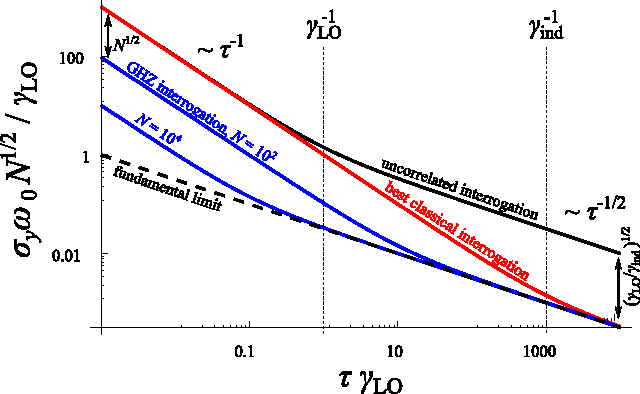
\includegraphics[width=0.9\textwidth]{./figs_Kessler2014/fig1.pdf}
\caption
[Comparison of clock protocols] 
{
\label{fig:sigma_tau}
Allan deviation $\sigma_y$ for different protocols as a function of averaging
time $\tau$, normalized to the standard quantum limit, for $\gamma_\mathrm{LO} /
\gamma_\mathrm{ind} = 10^3$. The solid black line corresponds to the standard scheme using
a single uncorrelated ensemble. It fails to reach the fundamental noise floor
set by the atomic transition linewidth (cf. \refeq{eq:sigma(2)}, broken line).
A more sophisticated classical scheme which uses exponentially increasing Ramsey
times in each cycle \cite{Rosenband2013, Borregaard2013} allows to extend the
regime of linear scaling with $1/\tau$ up to the point where the bound
(\ref{eq:sigma(2)}) is met. In comparison, the proposed cascaded GHZ protocol
(blue solid curves) enables an $\sim N$ times faster convergence. For short
averaging times the stability is enhanced by a factor $\sqrt{N}$ as compared to
classical protocols.
}
\end{figure} 


% 
% , where
% \bel
% 	\label{eq:S^2}
% 	S^2(\gamma T,C) = \frac{1}{\gamma T} C 
% 	+ \sqrt{32\pi}	\exp\left[-\frac{\pi^2}{2(\gamma T)^2}\right],
% \eel
% and
% \bel
% 	\label{eq:C}
% 	C(D,M,N) = \frac{1}{N D^{M-1}} +
% 	\frac{8\pi
% 	N^{1/2}}{D^{\frac{M+1}{2}}}\exp\left[-\frac{\pi^2 N}{2D^{M+1}}\right],
% \eel
% which can be obtain by approximating the
% integrals of the Gaussians with the first term of the asymptotic series,
%  $\int_x^\infty \d{\xi}\exp[-\xi^2/2] = \exp[-x^2/2]\left(1/x +
% \mathcal{O}(x^{-2})\right)$, and assuming $\sum_{j=0}^{M-1}D^j \approx D^{M-1}$.
% % Appendix \ref{sec:Optimization} contains the details of carrying out the
% % optimization.
% 
% The highest stability is achieved for the minimal $S^2$, which can be found by
% direct optimization, which we carry out in three steps.
% First, we find $\gamma T_\mathrm{opt}$ in terms of $C$, by finding the global
% minimum of \refeq{eq:S^2} analytically, in the limit $\gamma T \ll 1$, using the
% general solution of the transcendental equation $x^n = A\exp[-1/x]$ in the case
% of $A\gg 1$ (see Supplementary Materials).
% This yields $\gamma T_\mathrm{opt} =
% \frac{\pi}{\sqrt{2}}\left[\log\frac{8\pi^{3/2}}{C}\right]^{-1/2}$.
% The resulting function $S^2( \gamma T_\mathrm{opt}(C), C)$ is monotonically
% decreasing for $C \ll 1$, which is the relevant region for us.
% In the second step, we find $D_\mathrm{opt}$ in terms of $M$ and $N$ by finding
% the global minimum of \refeq{eq:C} analytically in the limit $N/D^{M+1} \gg 1$,
% using the same technique.
%%%%%%%%%%%%%%%%%%%%%%%%%%%%%%%%%%%%%%%%%%%%%%%%%%%%%%%%%%%%%%%%%%%%%%%%%%%%%%%%%%5
%%%%%%%%%%%%%%%%%%%%%%%%%%%%%%%%%%%%%%%%%%%%%%%%%%%%%%%%%%%%%%%%%%%%%%%%%%%%%%%%%%5
%\section{Different timescales}
\section{Comparison with other schemes}
%%%%%%%%%%%%%%%%%%%%%%%%%%%%%%%%%%%%%%%%%%%%%%%%%%%%%%%%%%%%%%%%%%%%%%%%%%%%%%%%%%5
%%%%%%%%%%%%%%%%%%%%%%%%%%%%%%%%%%%%%%%%%%%%%%%%%%%%%%%%%%%%%%%%%%%%%%%%%%%%%%%%%%5
%{\it Comparison with other schemes.}---
In the following, we benchmark the stability of our protocol against different approaches by
comparing the lowest achievable ADEV as a function of averaging
time $\tau$ (cf. \reffig{fig:sigma_tau}). 
First, we consider the standard procedure in which all atoms are interrogated
in an uncorrelated fashion. The scheme is identical to $N$
independent measurements of $\Phi_\mathrm{LO}$, and therefore the  ADEV
is limited by the standard quantum limit: $\sigma_y \sim \frac{1}{\omega_0
\tau\sqrt{N}}$ for $\tau < \gamma_\mathrm{LO}^{-1}$.
Since the Ramsey time is limited, by the LO noise, to $T<\gamma_\mathrm{LO}^{-1}$
due to uncorrected phase wraps, this fails to achieve the
fundamental bound, \refeq{eq:sigma(2)}, giving suboptimal ADEV,
  $\sigma_y(\tau) \sim
\frac{1}{\omega_0}\sqrt{\frac{\gamma_\mathrm{LO}}{\tau N}}$, in the long time
limit $ \tau > \gamma_\mathrm{LO}^{-1}$.
Second, we discuss the recently published classical protocol which
interrogates the LO with uncorrelated atoms for exponentially increasing Ramsey
times in each cycle \cite{Borregaard2013, Rosenband2013}. This protocol can be
understood as the classical part ($j\leq0$) of the cascaded interrogation
proposed here .
It eliminates the constraint of the LO linewidth, and allows to extend the interrogation time $T$ to its maximum value, enabling a linear scaling with $\tau$ up to the point where the fundamental bound
(\ref{eq:sigma(2)}) is reached.
However, using an uncorrelated interrogation, the scheme displays a standard-quantum-limited scaling (i.e.
$\propto1/\sqrt{N}$), for short averaging times. 
 
The above analysis illustrates the quantum gain of the proposed clock
operation protocol using cascaded GHZ states. As compared to the best known
classical scheme, our scheme provides a $\sqrt{N/\mathrm{log}(N)}$ enhancement for
short averaging times. As a result it reaches the fundamental noise floor for
laser stability in the presence of single particle decoherence
[\refeq{eq:sigma(2)}] $\sim N/{\mathrm{log}(N)}$ times faster.
This results identifies the possible advantage of using entanglement
previously debated in the literature
\cite{Wineland1998,Huelga1997,LouchetChauvet:2010fs,Rosenband2012_numerical,Borregaard2013_nearHeisenberg,Andre2004,Buzek1999,Meiser:2008fo}:
While the long term limitation is set by atomic decoherence, entangled atoms
reaches this limit faster thus improving the bandwidth of the stable oscillator.
Our results motivate the development of quantum enhanced atomic clocks based on entangled ions
and neutral atoms. Furthermore, it lays the foundations for the recently proposed network of quantum clocks \cite{Komar2014}
which achieves the optimal use of resources in a global network through
network-wide entangled states.

